

\label{XPS_theory}
\section{X-ray photoelectron spectroscopic analysis}
\subsection{Principle of measurement}


Photoelectron spectroscopy (PES) hinges on the fundamental principle of the photoelectric effect  as elucidated through the photon theory by Einstein and Rutherford \cite{rutherford_xxxvii_1914, einstein_uber_1905}. This concept essentially explains how incident light hitting a material results in the emission of electrons, known as photoelectrons.
In X-ray photoelectron spectroscopy, soft x-rays are commonly generated by exciting Aluminum or Manganese to radiate K \(\alpha\) x-rays with 1486.6 eV and 1253.6 eV respectively. These x-ray sources have a small natural linewidth and thus can provide high resolution. The produced photons then interact with the sample which in turn emit electrons, making use of the photoelectric effect previously described. Those electrons are then transported to a multichannel detector which counts the electrons. To improve, detector efficiency and electron collection, and thus the resolution, a monochromator is usually used.\cite{stevie_introduction_2020} The concept of the measurement can be expressed as shown in eq. 1:
\begin{equation}
    hv = BE + KE + \psi spec
\end{equation}
which can be re-arranged to express the binding energy as a function of known variables \cite{stevie_introduction_2020} as shown in eq. 2
\begin{equation}
    BE = hv- KE - \psi spec
\end{equation}



\begin{figure}
    \centering
    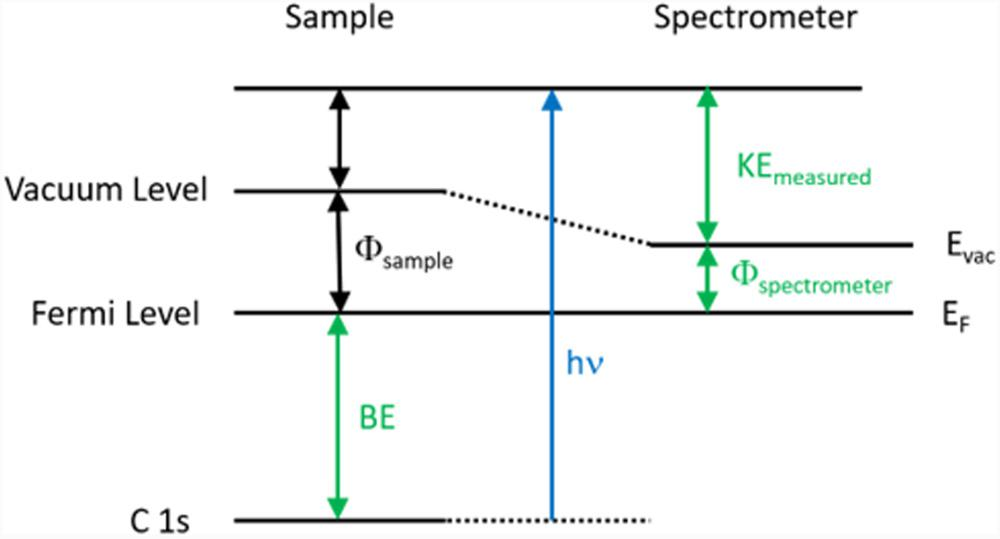
\includegraphics[width=0.7\textwidth]{Figures/image4_3.jpeg}
    \caption{}
    \label{fig:enter-label}
\end{figure}



The sample work function is a specific change in energy levels dependent on the chemical environment (coordination, charge etc.) of the atom of interest. It describes the work an electron must overcome to escape the local environment up to the vacuum level. 



The intensity of the peaks is indicated as counts and corresponds to the number of electrons that reach the detector during the acquisition time. Thus, the intensity of the signal depends on the acquisition time and should be normalized before comparing with spectra collected with unknown method and instrument parameters.
The complex and sample-specific interactions of the produced electrons with the sample are discussed in the next subchapter.

\subsection{Peaks origin} % identification?

As X-ray photoelectron spectroscopy uses x-rays to produce core-level electrons from a sample, the detection of these electrons is the desired origin of a so-called photoelectron peak. However, XPS measurements always show additional peaks from other origins. The different peak origins are listed and discussed subsequently.

\subsubsection{Auger electron peaks}

When a core electron is lost due to the X-ray excitation, a deficiency of electrons results. This ionized state is then relaxed with an electron from the outer-most so-called valence orbital \cite{stevie_introduction_2020}. This process induces the release of energy which can then be detected with XPS. It is crucial to note that this process is independent of the source energy and thus, Auger peak positions will move as another source of X-rays is used. This is especially important to resolve issues when Auger peaks overlap with photoelectron peaks. 

\subsubsection{Shakeup peaks}

While an electron is travelling towards the detector, it might interact with valence electrons of other atoms and lose some of its energy. This process is an energy-loss process and thus, the peak observed is shifted 

\subsubsection{Plasmon peaks}


\subsubsection{Multiplet splitting}


\subsection{Surface sensitivity}

The study of surface sensitivity in XPS has been thoroughly studied and summarized in multiple publications \cite{powell_surface_2009, }. Electrons emitted from the samples atoms can take different ways until they reach the detector. They either take a direct path (A), are elastically scattered and return to the detector (B) or are inelastically scattered and do not return to the detector.




To this point, there are three terms to describe surface sensitivity in XPS.
\begin{itemize}
\item The initial energy which is needed to overcome dielectric effects such that an electron can be lost from a material is described by the electron loss function (ELF)
\item Inelastic mean free path (IMFP), often denoted as $\lambda$, describes the distance an electron travels in a given material before inelastically scattering.
\item Electron attenuation length (EAL) is the length the electron travels into the sample.

\end{itemize}

\begin{figure}
    \centering
    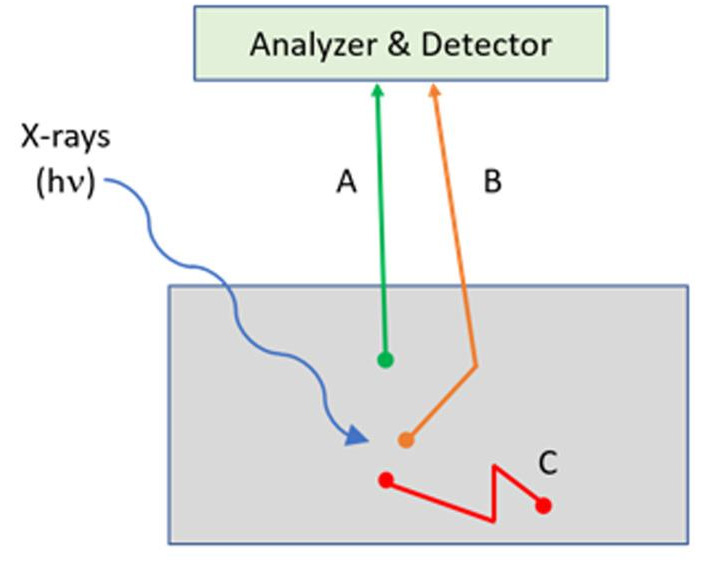
\includegraphics[width=0.3\textwidth]{Figures/image6_1.jpg}
    \caption{Scattering effects in XPS \cite{stevie_introduction_2020}}
    \label{fig:scattering}
\end{figure}

Elastic electron scattering, however, has often caused uncertainties in measurements of EAL and IMFP. 
The IMFP is element specific and also depends on the kinetic energy. 


\subsection{Adventitious Carbon}

When analyzing with XPS, we often find peaks which do not originate from the sample but from the atmosphere. As the atmosphere consists of organic compounds, they include O 1s and C 1s peaks. Often, the C 1s peak is used as a internal standard reference peak to shift the measured spectra to the correct position. This is done because peak shifts occur frequently owing to charging effects which arise from sample properties. Due to varying atmospheric composition, however, this peaks' position is uncertain and is itself  not clearly defined. \cite{biesinger_accessing_2022} As the peak reference to adventitious carbon is most frequently used, it should be considered when comparing, evaluating and analysing experimental data.

\subsection{Depth profiling}

Experimentally, there exist four methods for investigating depth-information of a component in a sample. These are:
\begin{enumerate}
    \item presence or absence of energy loss peaks which occur when electrons from deeper regions of the material need to travel to the surface and lose energy (associated to the elastic scattering effect)
    \item the intensity ratio of peaks across the kinetic energy (high vs low) – only suitable for a selection of elements (semi-qualitative).
    \item controlled erosion and subsequent measurement of the surface (destructive and high material dependency)
    \item measurement at different sample-mounting angles (ARXPS). \cite{moulder_handbook_1992} 
    \end{enumerate}
and more recently have been extended by two additional methods:
\begin{enumerate}[resume]
    \item Combination with hard x-ray photoelectron spectroscopy (HAXPES) has become more accessible which in combination with XPS can give depth information of a sample \cite{zborowski_improved_2022}.
    \item Modelling of X-ray photoelectron spectra another recent technique for the determination of depth distribution and has been investigated previously using manual approaches \cite{zborowski_comparison_2022}.

\end{enumerate}


The methods 1-3 have the drawback of being potentially destructive on the sample surface. Further, they are giving only very vague information about the samples’ depth profile; the accuracy is often denoted to be $\pm$10\%.
The non-destructive methods 4-6 (ARXPS / Modelling / XPS-HAXPES) are further explained, as they are comparable to our data-driven approach.

\subsubsection{Angle resolved XPS (ARXPS)}

A variation on the XPS-technique involves measurements at different mounting-angles of the sample.
This changes the path the X-rays take into and out from the sample, as shown in Figure \ref{fig:arxps} which compares a standard 90\textdegree  take-off angle (a) with a smaller angle $\alpha$ (b). As the angle $\alpha$ decreases, the X-rays travel through a proportional higher amount of surface which in turn increases the sensitivity towards the surface. From the obtained spectra (c), we can deduct the surface composition and - if 

\begin{figure}
    \centering
    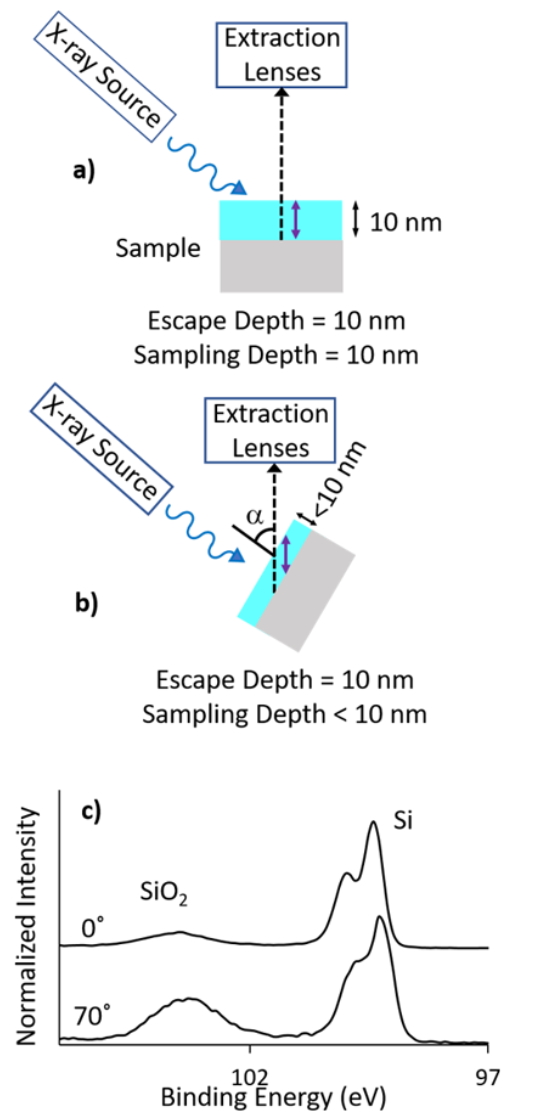
\includegraphics[width=0.4\textwidth]{Figures/ARXPS.png}
    \caption{Angle resolved XPS \cite{stevie_introduction_2020}}
    \label{fig:arxps}
\end{figure}


\subsubsection{XPS-HAXPES}

Hard X-ray photoelectoron spectroscopy is a technique similar to XPS, but it uses hard x-ray sources from Gallium or Chromium to achieve much higher energy levels. As these X-rays are in the range of multiple keVs, the IMFP increases drastically and we are able to probe much deeper into the surface compared to XPS. Combining the two analyses can provide researchers with valuable information of the surface and the deeper regions of samples. This approach has been demonstrated to be accurate in multiple publications \cite{bure_assessing_2023, siol_concepts_2020} 